\section{Различия между MapReduce и Spark.}

В MapReduce после каждой итерации происходит запись
результата на диск, в то время как Spark между итерациями
сохраняет данные в памяти, что ускоряет работу.

\begin{figure}[H]
	\centering
	\begin{minipage}[b]{0.8\textwidth}
		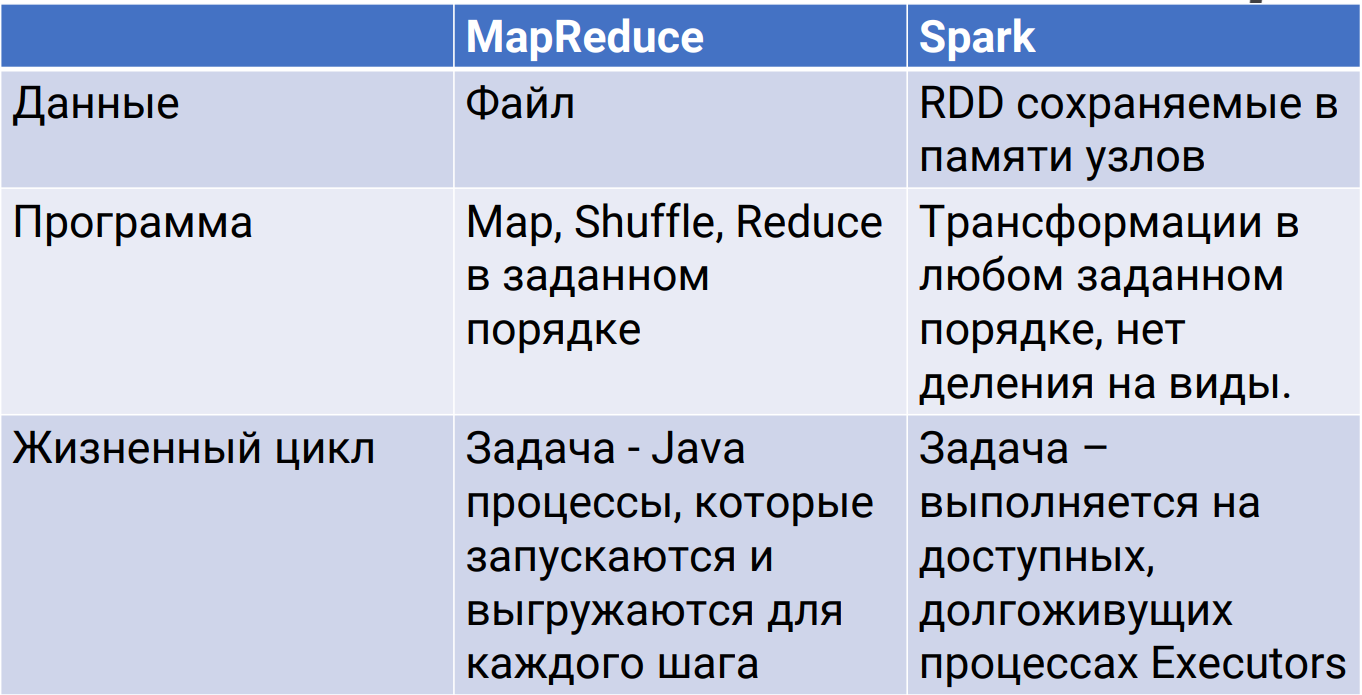
\includegraphics[width=\textwidth]{images/mrvspark.png}
		\caption{MR vs Spark}
	\end{minipage}
\end{figure}

MapReduce каждый шаг запускает и удаляет процессы Mapper
и Reducer.

Spark - каждый Executor является долгоживущим процессом,
в течение жизни может исполнять несколько задач последовательно
или параллельно.